\documentclass{article}
\usepackage{amsfonts,amsmath,amssymb,amsthm}
\usepackage{subfigure}
\usepackage{wrapfig}
\usepackage{sidecap}
\usepackage{algorithm,algorithmic}
\usepackage[usenames,dvipsnames,pdftex]{color}
\usepackage[colorlinks=true,linkcolor=magenta]{hyperref}
\usepackage[sort&compress,colon,square,numbers]{natbib}
\usepackage{soul}
\usepackage[pdftex,dvips]{graphicx}
\usepackage{boxedminipage}
\usepackage{amsfonts}
\usepackage{amsmath}
\usepackage{url}
\usepackage[table]{xcolor}
\usepackage[normalem]{ulem}
\usepackage{comment}
\usepackage{paralist}
\usepackage{chngcntr}
\usepackage{caption}% http://ctan.org/pkg/caption
\usepackage{etoolbox}% http://ctan.org/pkg/etoolbox
\usepackage{mparhack} 
\usepackage{multirow}
\usepackage{booktabs}
\usepackage{fancyhdr}

\usepackage[left,pagewise]{lineno}  %%Get rid of indenting throughout entire document

  % \presetkeys{todonotes}{fancyline, color=blue!30}{}

\newcommand{\mytodo}[1]{\marginpar{\textcolor{red}{{\small TODO: #1}}}}

\captionsetup{font=small}


% \counterwithin{figure}{section}


\definecolor{MyPlum}{rgb}{0.3,0,0.3}
\definecolor{MyOrange}{rgb}{1,0.5,0}
\definecolor{deep_blue}{rgb}{0,.2,.5}
\definecolor{dark_blue}{rgb}{0,.15,.5}
\usepackage[linecolor=dark_blue, linewidth=1.5pt, skipabove=4pt, nobreak=true]{mdframed}

  % 
% \hypersetup{pdftex,  % needed for pdflatex
%   breaklinks=true,  % so long urls are correctly broken across lines
%   colorlinks=true,
%   linkcolor=dark_blue,
%   citecolor=deep_blue,
% }
% 

\newcommand{\db}[1]{{\color{dark_blue}{#1}}}
\newcommand{\bb}[1]{{\textbf{\db{#1}}}}

% 
% 
\newcommand{\randal}[1]{{\color{orange}{\it RB: #1}}}
\newcommand{\jovo}[1]{{\color{red}{\it JoVo: #1}}}
\newcommand{\cep}[1]{{\color{blue}{\it cep: #1}}}
\newcommand{\markc}[1]{{\color{green}{\it mark: #1}}}
\newcommand{\da}[1]{{\color{yellow}{\it da: #1}}}
\newcommand{\disa}[1]{{\color{purple}{\it disa: #1}}}
\newcommand{\will}[1]{{\color{cyan}{\it will: #1}}}
\newcommand{\kunal}[1]{{\color{magenta}{\it kunal: #1}}}
\newcommand{\alex}[1]{{\color{MyPlum}{\it alex: #1}}}
\newcommand{\vince}[1]{{\color{deep_blue}{\it vince: #1}}}
\newcommand{\minh}[1]{{\color{NavyBlue}{\it minh: #1}}}
\newcommand{\priya}[1]{{\color{Lavender}{\it priya: #1}}}
\newcommand{\jason}[1]{{\color{red}{\it jason: #1}}}

% \newcommand{\annotation}[1]{%
%   \marginpar{\addfontfeature{Color=0000FF}\small\itshape#1}}

% 
% \newcommand{\sectn}[1]{\section{#1} \rfoot{\small #1 ~~ \thepage}}
% %\newcommand{\sectn*}[1]{\section*{#1} \rfoot{\small #1 ~~ \thepage}}
% 
% \renewcommand{\thepage}{\thesection-{\arabic{page}}}
\renewcommand{\thesection}{\Roman{section}}   % set the section counter to Alpha
\renewcommand{\thesubsection}{\Roman{section}.\Alph{subsection}}   % set the subsection counter to alpha
% \renewcommand{\thesubsubsection}{\Alph{section}.\arabic{subsection}(\arabic{subsubsection})}   % set the subsection counter to alpha
% 
% 
\makeatletter
% \def\subsize{\@setsize\subsize{8pt}\xipt\@xipt}
 \def\section{\@startsection {section}{1}{\z@}{5pt}{9pt}{\Large\bf\db}}
 \def\subsection{\@startsection {subsection}{2}{\z@}{10pt}{4pt}{\large\bf\db}}
 \def\subsubsection{\@startsection {subsubsection}{2}{\z@}{10pt}{4pt}{\bf\db}}
% \def\subs{\@startsection {subsubsection}{2}{0pt}{5pt}{0pt}{ \subsize\bf\db}}
\def\paragraph{\@startsection {paragraph}{2}{\z@}{10pt}{4pt}{\bf\db}}
% \def\subparagraph{\@startsection {subparagraph}{2}{\z@}{10pt}{4pt}{\qquad \bf\db}}
\newcommand{\para}[1]{\vspace{3pt}\noindent{\bf \db{#1}}}
\newcommand{\subpara}[1]{\vspace{0pt}\qquad{\bf \db{#1.}}}% \newcommand{\paranc}[1]{\vspace{0pt}\noindent{\bf #1}}
% \makeatother
% 
% 

\pagestyle{fancy}
% \fancyhf{} % sets both header and footer to nothing
% \renewcommand{\headrulewidth}{0pt}
% \setlength{\parindent}{0in}
% \setlength{\parskip}{3pt}
\setlength{\voffset}{-1in}


% % \setlength{\abovedisplayskip}{-5pt}
% % \setlength{\belowdisplayskip}{-15pt}
% % \setlength{\abovedisplayshortskip}{-15pt}
% % \setlength{\belowdisplayshortskip}{-5pt}
% % \baselineskip=0pt
% % \abovedisplayskip=0.7cm
% % \abovedisplayshortskip=-0.3cm
% % \belowdisplayskip=0.7cm
% % \belowdisplayshortskip=0.4cm
% % % \setlength{\voffset}{-15pt}
% % % \setlength{\headsep}{15pt}
% % % \setlength{\textheight}{9.5in}
% % \setlength{\belowcaptionskip}{0pt}

\setlength{\textheight}{9.5in}
\setlength{\textwidth}{6.5in}

% \setlength{\leftmargin}{-1in}
% \setlength{\rightmargin}{2in}
\setlength{\oddsidemargin}{0in}
% \setlength{\evensidemargin}{1in}

\pagenumbering{arabic}
\setlength{\tabcolsep}{1pt}

% \linenumbers
% \usepackage[utf8]{inputenc}
 

% \setlength{\textheight}{10in}
% \setlength{\topmargin}{-15pt}
% 
% \newlength{\saveparindent}
% \setlength{\saveparindent}{\parindent}
% \newlength{\saveparskip}
% \setlength{\saveparskip}{\parskip}
% 
% \newenvironment{newenumerate}{%
% \begin{list}{{\rm \arabic{ctr}.}\hfill}{\usecounter{ctr}\labelwidth=17pt%
% \labelsep=6pt \leftmargin=23pt \topsep=.5pt%
% \setlength{\listparindent}{\saveparindent}%
% \setlength{\parsep}{\saveparskip}%
% \setlength{\itemsep}{5pt} }}{\end{list}}
% 
% \newenvironment{newitemize}{%
% \begin{list}{\hspace{3pt}$\bullet$\hfill}{\labelwidth=12pt%
% \labelsep=3pt \leftmargin=15pt \topsep=1pt%
% \setlength{\listparindent}{\saveparindent}%
% \setlength{\parsep}{\saveparskip}%
% \setlength{\itemsep}{1pt}}}{\end{list}}
% 
% 
\pagestyle{plain}
% % \lhead{}
% % \chead{}
% % \rhead{}
% % \lfoot{}
% % \cfoot{}
% % \rfoot{}
% % \renewcommand{\headrulewidth}{0pt}
% % \renewcommand{\footrulewidth}{0pt}
% 
% \tolerance=1000
% 
% % \setupheads[indentnext=yes]

%%%%%%%%%%%%%%%%%%%%%%%%%%%%%%%%%%%%



%%%%%%% Two column control
\newif\ifdotwocol
\dotwocoltrue   % two col
%\dotwocolfalse   % one col
\long\def\twocol#1#2{\ifdotwocol{#1}\else{#2}\fi}
%%%%%%%

\def\mybeforeequation{\footnotesize}
%\def\mybeforeequation{\small}
%\def\mybeforeequation{}

\def\myafterequation{\renewcommand\baselinestretch{1.1}}
%\def\myafterequation{}

%%%%%%%%%%%%%%%%
%%%%%%%%%%%%%%%%

\def\citeusmark{$^{\textstyle \star}$}
\def\citeus#1#2{\cite{#1}}

\def\crow#1#2{#2}


\def\Paper{grant application}
\def\paper{application}
\def\refappendix{Sec.}

\def\poster{(Poster)}

%Note from brd
\long\def\todo#1{{\bf{To do:}} #1}
%\long\def\todo#1{}
\def\ICRA{IEEE International Conference on Robotics and Automation (ICRA)}

\long\def\squeezable#1{#1}

%\def\a5{$\alpha_{_5}$

\def\a5{5}

%\def\mycaptionsize{\normalsize}
%\def\mycaptionsize{\small}
%\def\mycaptionsize{\small}
\def\mycaptionsize{\footnotesize}
\def\mycodesize{\footnotesize}
\def\myeqnsize{\small}

\def\sheading#1{{\bf #1:}\ }
\def\sheading#1{\subsubsection{#1}}
%\def\sheading#1{\bigskip {\bf #1.}}

\def\ssheading#1{\noindent {\bf #1.}\ } 

\newtheorem{hypothesis}{Hypothesis}
\long\def\hyp#1{\begin{hypothesis} #1 \end{hypothesis}}

\def\cbk#1{[{\em #1}]}

\def\R{\mathbb{R}}
\def\midv{\mathop{\,|\,}}
\def\Fscr{\mathcal{F}}
\def\Gscr{\mathcal{G}}
\def\Sscr{\mathcal{S}}
\def\set#1{{\{#1\}}}
\def\edge{\!\rightarrow\!}
\def\dedge{\!\leftrightarrow\!}
\newcommand{\EOP}{\nolinebreak[1]~~~\hspace*{\fill} $\Box$\vspace*{\parskip}\vspace*{1ex}}
%my way of doing starred references
\newcommand{\mybibitem}[1]{\bibitem{#1} 
\label{mybiblabel:#1}}
\newcommand{\BC}{[}
\newcommand{\EC}{]}
\newcommand{\mycite}[1]{\ref{mybiblabel:#1}\nocite{#1}}
\newcommand{\starcite}[1]{\ref{mybiblabel:#1}\citeusmark\nocite{#1}}


\def\degree{$^\circ$}
\def\R{\mathbb{R}}
\def\Fscr{\mathcal{F}}
\def\set#1{{\{#1\}}}
\def\edge{\!\rightarrow\!}
\def\dedge{\!\leftrightarrow\!}

\long\def\gobble#1{}
\def\Jigsaw{{\sc Jigsaw}}
\def\ahelix{\ensuremath{\alpha}-helix}
\def\ahelices{\ensuremath{\alpha}-helices}
\def\ahelical{$\alpha$-helical}
\def\bstrand{\ensuremath{\beta}-strand}
\def\bstrands{\ensuremath{\beta}-strands}
\def\bsheet{\ensuremath{\beta}-sheet}
\def\bsheets{\ensuremath{\beta}-sheets}
\def\hone{{\ensuremath{^1}\rm{H}}}
\def\htwo{{$^{2}$H}}
\def\cthir{{\ensuremath{^{13}}\rm{C}}}
\def\nfif{{\ensuremath{^{15}}\rm{N}}}
\def\hn{{\rm{H}\ensuremath{^\mathrm{N}}}}
\def\hnone{{\textup{H}\ensuremath{^1_\mathrm{N}}}}
\def\ca{{\rm{C}\ensuremath{^\alpha}}}
\def\catwel{{\ensuremath{^{12}}\rm{C}\ensuremath{^\alpha}}}
\def\ha{{\rm{H}\ensuremath{^\alpha}}}
\def\cb{{\rm{C}\ensuremath{^\beta}}}
\def\hb{{\rm{H}\ensuremath{^\beta}}}
\def\hg{{\rm{H}\ensuremath{^\gamma}}}
\def\dnn{{\ensuremath{d_{\mathrm{NN}}}}}
\def\dan{{\ensuremath{d_{\alpha \mathrm{N}}}}}
\def\jconst{{\ensuremath{^{3}\mathrm{J}_{\mathrm{H}^{\mathrm{N}}\mathrm{H}^{\alpha}}}} }
\def\cbfb{{CBF-$\beta$}}

\newtheorem{defn}{Definition}
\newtheorem{claim}{Claim}

    \gobble{
    \psfrag{CO}[][]{\colorbox{white}{C}}
    \psfrag{OO}[][]{\colorbox{white}{O}}
    \psfrag{CA}[][]{\colorbox{white}{\ca}}
    \psfrag{HA}[][]{\colorbox{white}{\ha}}
    \psfrag{CB}[][]{\colorbox{white}{\cb}}
    \psfrag{HB}[][]{\colorbox{white}{\hb}}
    \psfrag{HN}[][]{\colorbox{white}{\hn}}
    \psfrag{N15}[][]{\colorbox{white}{\nfif}}
    \psfrag{dnn}[][]{\dnn}
    \psfrag{dan}[][]{\dan}
    \psfrag{phi}[][]{$\phi$}
    }

\newenvironment{closeenumerate}{\begin{list}{\arabic{enumi}.}{\topsep=0in\itemsep=0in\parsep=0in\usecounter{enumi}}}{\end{list}}
\def\CR{\hspace{0pt}}           % ``invisible'' space for line break



\newif\ifdbspacing
%\dbspacingtrue  % For double spacing
\dbspacingfalse  % For normal spacing

\ifdbspacing
 \doublespacing
 \newcommand{\capspacing}{\doublespace\mycaptionsize}
\else
 \newcommand{\capspacing}{\mycaptionsize}
\fi

\def\rulefigure{\smallskip\hrule}

% \def\codesize{\normalsize}
\def\codesize{\small}

% Can use macros \be, \ee, \en as shortcuts
%  for \begin{enumerate}, \end{enumerate}, \item
%  respectively.

\newtheorem{proposition}{Proposition}
\newtheorem{lemma}{Lemma}

\setlength{\fboxrule}{1pt}%
\setul{}{1.0pt}

%%%%%%%%%%%%%%%%%%%%%%%%%%%%%%%%%%

\makeatletter
% \renewcommand{\labelitemi}{*}


% \providecommand{\tg}[1]{\textcolor{green}{#1}}
% \providecommand{\tb}[1]{\textcolor{blue}{#1}}
% \providecommand{\tr}[1]{\textcolor{red}{#1}}
% \providecommand{\tk}[1]{\textcolor{black}{#1}}
% \providecommand{\twhite}[1]{\textcolor{white}{#1}}
% \providecommand{\ve}[1]{\boldsymbol{#1}}
% \providecommand{\ma}[1]{\boldsymbol{#1}}
\providecommand{\norm}[1]{\left \lVert#1 \right  \rVert}
% \providecommand{\deter}[1]{\lvert #1 \rvert}
\providecommand{\abs}[1]{\left \lvert #1 \right \rvert}
% \providecommand{\mat}[1]{\left[ #1 \right]}
% \newcommand{\trans}[1]{{#1}^{\ensuremath{\mathsf{T}}}}           % transpose
% \newcommand{\transpose}[1]{{#1}^{\ensuremath{\mathsf{T}}}}           % transpose
\newcommand{\argmax}{\operatornamewithlimits{argmax}}
\newcommand{\argmin}{\operatornamewithlimits{argmin}}
\newcommand{\T}{^{\ensuremath{\mathsf{T}}}}           % transpose
\newcommand{\from}{{\ensuremath{\colon}}}           % :

\newcommand{\Aa}{\mathbb{A}}
\newcommand{\BB}{\mathbb{B}}
\newcommand{\CC}{\mathbb{C}}         
\newcommand{\DD}{\mathbb{D}}         
\newcommand{\EE}{\mathbb{E}}           % expected value
\newcommand{\FF}{\mathbb{F}}         
\newcommand{\GG}{\mathbb{G}}
\newcommand{\HH}{\mathbb{H}}         
\newcommand{\II}{\mathbb{I}}           % indicator function
\newcommand{\LL}{\mathbb{L}}
\newcommand{\MM}{\mathbb{M}}
\newcommand{\NN}{\mathbb{N}}
\newcommand{\PP}{\mathbb{P}}         
\newcommand{\QQ}{\mathbb{Q}}           
\newcommand{\SSS}{\mathbb{S}}           
\newcommand{\VV}{\mathbb{V}}
\newcommand{\XX}{\mathbb{X}}         
\newcommand{\YY}{\mathbb{Y}}
\newcommand{\ZZ}{\mathbb{Z}}         

\newcommand{\iid}{\overset{iid}{\sim}}
\newcommand{\knn}{$k$NN}

% \DeclareMathOperator{\find}{find}

\newtheorem{thm}{Theorem}
\newcommand{\thma}{\begin{thm}}
\newcommand{\thmb}{\end{thm}}

\newcommand{\mata}{\begin{bmatrix}}
\newcommand{\matb}{\end{bmatrix}}


\newcommand{\bth}{\ve{\theta}}
\newcommand{\hth}{\mh{\theta}}
\newcommand{\htth}{\mh{\theta}}
\newcommand{\bhth}{\mh{\ve{\theta}}}
\newcommand{\thetn}{\ve{\theta}}
\newcommand{\thet}{\thetn}
\newcommand{\theth}{\widehat{\ve{\theta}}}
\newcommand{\theto}{\ve{\theta}'}
\newcommand{\wht}{\widehat{\thet}}
\newcommand{\wtt}{\widetilde{\thet}}
\newcommand{\vth}{\ve{\thet}}
\newcommand{\vTh}{\ve{\Theta}}
\newcommand{\hvth}{\widehat{\ve{\thet}}}
\newcommand{\bTh}{\ve{\Theta}}
\newcommand{\hbth}{\widehat{\thet}}
\newcommand{\tbth}{\tilde{\bth}}

% \newcommand{\p}{P_{\bth}}
\newcommand{\pold}{P_{\bth'}}
\newcommand{\pk}{P_{\widehat{\ve{\theta}}^{(k)}}}
\newcommand{\pT}{P_{\thetn_{Tr}}} %\thetn_T
\newcommand{\pO}{P_{\thetn_o}} %\thetn_o
% \newcommand{\Q}{Q(\thetn,\theto)}
% \newcommand{\m}{m^{\ast}}
% \newcommand{\q}{q(\ve{H}_t)}
\newcommand{\Ca}{[\text{Ca}^{2+}]}

\newcommand{\Lik}{\mathcal{L}}
\newcommand{\Cae}{[\widehat{\text{Ca}}^{2+}]}
\newcommand{\Cav}{\ve{C}}%[\ve{\text{Ca}}^{2+}]}
\newcommand{\sml}{\sqrt{\ma{\lambda}}}
\newcommand{\ml}{\ma{\lambda}}
\newcommand{\nw}{\widehat{n}}
\newcommand{\nv}{\vec{n}}
\newcommand{\Ae}{\widehat{A}}
\newcommand{\te}{\widehat{\tau}}
\newcommand{\maxn}{\max_{\ve{n}: n_t \geq 0}}
% \newcommand{\V}{\text{Var}}

\providecommand{\ms}[1]{\mathsf{#1}}
\providecommand{\mc}[1]{\mathcal{#1}}
\providecommand{\mb}[1]{\boldsymbol{#1}}
\providecommand{\mbb}[1]{\mathbb{#1}}
\providecommand{\mv}[1]{\vec{#1}}
\providecommand{\mh}[1]{\hat{#1}}
\providecommand{\wh}[1]{\widehat{#1}}
\providecommand{\mhv}[1]{\mh{\mv{#1}}}
\providecommand{\mvh}[1]{\mv{\mh{#1}}}
\providecommand{\mt}[1]{\widetilde{#1}}
\providecommand{\mhc}[1]{\hat{\mathcal{#1}}}
\providecommand{\mbc}[1]{\mb{\mathcal{#1}}}
\providecommand{\mvc}[1]{\mv{\mathcal{#1}}}
\providecommand{\mtc}[1]{\widetilde{\mathcal{#1}}}
\providecommand{\mth}[1]{\mt{\mh{#1}}}
\providecommand{\mht}[1]{\mh{\mt{#1}}}
\providecommand{\mhb}[1]{\hat{\boldsymbol{#1}}}
\providecommand{\whb}[1]{\widehat{\boldsymbol{#1}}}
\providecommand{\mvb}[1]{\vec{\boldsymbol{#1}}}
\providecommand{\mtb}[1]{\widetilde{\boldsymbol{#1}}}

\newcommand{\PmcP}{P \in \mc{P}}
\newcommand{\mP}{\mathbb{P}}

\newcommand{\del}{\delta}
\newcommand{\sig}{\sigma}
\newcommand{\lam}{\lambda}
\newcommand{\gam}{\gamma}
\newcommand{\eps}{\varepsilon}

\newcommand{\Del}{\Delta}
\newcommand{\Sig}{\Sigma}
\newcommand{\Lam}{\Lambda}
\newcommand{\Gam}{\Gamma}

\newcommand{\dvs}{\dot{\bs}_t}
\newcommand{\dvw}{\dot{\bw}_t}
\newcommand{\dvx}{\dot{\bx}_t}
\newcommand{\dvy}{\dot{\by}_t}

\newcommand{\ft}{f_{\ve{\thet}}}
\newcommand{\gt}{g_{\ve{\thet}}}
\newcommand{\hht}{h_{\thetn}}

\newcommand{\Real}{\mathbb{R}}

\newcommand{\wconv}{\overset{i.p.}{\rightarrow}}
\newcommand{\sconv}{\overset{i.p.}{\rightarrow}}
\newcommand{\conv}{\rightarrow}
\newcommand{\pconv}{\overset{p}{\conv}}
\newcommand{\mcE}{\mathcal{E}}
\newcommand{\mcT}{\mathcal{T}}
\newcommand{\mcG}{\mathcal{G}}
\newcommand{\mcM}{\mathcal{M}}
\newcommand{\mcL}{\mathcal{L}}
\newcommand{\hatmcE}{\widehat{\mcE}}
\newcommand{\hatp}{\widehat{p}}
\newcommand{\hatP}{\widehat{P}}
\newcommand{\hatQ}{\widehat{Q}}
\newcommand{\hatL}{\widehat{L}}
\newcommand{\mhP}{\widehat{\PP}}
\newcommand{\tildeA}{\widetilde{A}}

\newcommand{\defa}{\begin{defi}}
\newcommand{\defb}{\end{defi}}
\newcommand{\defeq}{\overset{\triangle}{=}}


% \newcommand{\ss}{\mc{S}}
% \newcommand{\mhc}{\mh{\mc{S}}_n}

% \newcommand{\Real}{\mathbb{R}}
% \newcommand{\bTh}{\mb{\Theta}}
% \newcommand{\ra}{\rightarrow}
% \newcommand{\la}{\leftarrow}
\newcommand{\bX}{\mb{X}}

% \newcommand{\bv}{\mb{v}}
% \newcommand{\ba}{\mb{a}}
% \newcommand{\bd}{\mb{d}}
% \newcommand{\balpha}{\mb{\alpha}}
% \newcommand{\conv}{\rightarrow}  
% \newcommand{\xx}{\langle \bx_u^\la, \bx_v^\ra\rangle}  
% \DeclareMathOperator*{\argmax}{arg \hspace{1pt} max \hspace{2pt}}
% \DeclareMathOperator*{\argmin}{arg \hspace{1pt} min \hspace{2pt}}
% \newcommand{\norm}[1]{\left \lVert#1 \right  \rVert}
% 


% \newcommand{\theHalgorithm}{\arabic{algorithm}}


\DeclareMathOperator{\Delti}{\mathbf{\Delta}^{-1}}
\DeclareMathOperator{\Delt}{Q} %\mathbf{\Delta}}
% \DeclareMathOperator{\Gam}{\mathbf{\Gamma}}
\DeclareMathOperator{\Gami}{\mathbf{\Gamma}^{-1}}
\DeclareMathOperator{\Sigb}{\mathbf{\Sigma}}
\DeclareMathOperator{\Ri}{\mathbf{\R}^{-1}}
\DeclareMathOperator{\A}{A}
\DeclareMathOperator{\W}{\mathbf{W}}
\DeclareMathOperator{\V}{\mathbf{V}}
\DeclareMathOperator{\U}{\mathbf{U}}
\DeclareMathOperator{\C}{\mathbf{C}}
\DeclareMathOperator{\uvec}{\mathbf{u}}
\DeclareMathOperator{\D}{\mathbf{D}}
\DeclareMathOperator{\Q}{\mathbf{Q}}
% \DeclareMathOperator{\R}{R} %\mathbf{P}}
\DeclareMathOperator{\Y}{\mathbf{Y}}
\DeclareMathOperator{\B}{\mathbf{B}}
\DeclareMathOperator{\Hmat}{\mathbf{H}}
\DeclareMathOperator{\Gmat}{\mathbf{G}}
\DeclareMathOperator{\X}{\mathbf{X}}
\DeclareMathOperator{\Cmat}{C} %\mathbf{L}}
\DeclareMathOperator{\Pmat}{\mathbf{P}}
\DeclareMathOperator{\veta}{\mathbf{\mb{v}}}
\DeclareMathOperator*{\minimize}{\mathrm{minimize}}
\DeclareMathOperator*{\maximize}{\mathrm{maximize}}
\DeclareMathOperator*{\Ymod}{\mathbf{\Y}}
\DeclareMathOperator*{\Bmod}{\mathbf{B}}
\DeclareMathOperator*{\Hmod}{\mathbf{H}}
\DeclareMathOperator*{\Lmod}{\mathbf{L}}
\DeclareMathOperator*{\Xmod}{\mathbf{\X}}
% \DeclareMathOperator*{\mb{v}mod}{\mathbf{\mb{v}}}

\newcommand{\elegans}{\emph{C. elegans} }

\newcommand{\FAQ}{\texttt{FAQ} }

\providecommand{\tg}[1]{\textcolor{green}{#1}}
\providecommand{\tb}[1]{\textcolor{blue}{#1}}
\providecommand{\tr}[1]{\textcolor{red}{#1}}

\newcommand{\Qs}{Q}
\newcommand{\mcS}{\mc{S}}
\newcommand{\mcU}{\mc{U}}

\newcommand{\mbd}{\mb{d}}
\newcommand{\mbD}{\mb{D}}
\newcommand{\mbx}{\mb{x}}
\newcommand{\mbX}{\mb{X}}
\newcommand{\mby}{\mb{y}}
\newcommand{\mbY}{\mb{Y}}

\newcommand{\mtbd}{\mtb{d}}
\newcommand{\mtbD}{\mtb{D}}
\newcommand{\mtbx}{\mtb{x}}
\newcommand{\mtbX}{\mtb{X}}
\newcommand{\mtby}{\mtb{y}}
\newcommand{\mtbY}{\mtb{Y}}

% \floatname{algorithm}{Procedure}
% \renewcommand{\algorithmicrequire}{\textbf{Input:}}
% \renewcommand{\algorithmicensure}{\textbf{Output:}}
% \floatname{algorithm}{Pseudocode}

\providecommand{\sct}[1]{{\sc \texttt{#1}}}
\newcommand{\MMM}{M$^6$}
% multiple massive multi-scale, multi-spectral, multi-modal,  and multifarious


\title{\vspace{-50pt}
\db{Computational Analyses Supporting Diverse Synaptic Clusters}
}
\author{Adam Li, Tyler Tomita}


\begin{document}

\maketitle

\begin{abstract}
Currently, very little is understood about the synaptic connections within our brain. Our original belief is that there are only two types of synapses: excitatory and inhibitory. However, it is now known that there is a much more diverse synapse population. We want to characterize these different subpopulations. Here we present an analysis of Array Tomography data that supports hypotheses that there is a richer set of clusters then just excitatory and inhibitory. 
\end{abstract}

\section{Introduction}
Many hundreds of distinct proteins are involved in the development of synapses and mechanisms in synaptic signaling. Although complex, this molecular architecture can enable a better characterization of synaptic populations and subgroups based on protein clustering. We are aware of excitatory and inhibitory synapses, but it is now known there is a much more diverse populations \cite{Wheeler2015,Usoskin2014a}.

Differences in protein expression patterns at individual synapses could constitute a key to understanding synaptic diversity. The dataset was produced by Weiler, et al. using array tomography (ATomo) and the columnar organization of mouse barrel cortext with stains of over a dozen synaptic molecules \cite{Weiler2014}. 

ATomo is well suited to proteomic mapping of synaptic circuits because ultrathin sectionining of resin-embedded tissue samples enable immunohistochemical multiplexing and high-resolution imaging of millions of synapses \cite{Micheva2007}.

It is difficult to sift through millions of synaptic locations and determine subgroups by eye. With the development of increasing computational power and techniques, it is becoming easier to analyze large datasets and glean information on trends and clusters. Here, we employ a data driven approach to computationally analyze the synapse population of this dataset to glean insights into clusters and subclusters.

\section{Methods}
\subsection{Data}
Data was gathered from http://openconnecto.me/, the OpenConnectome project, and preprocessing was done to identify synapses based on the Synapsin expression levels in the ATomo pipeline \cite{Weiler2014}. The resulting dataset was a 1119299 x 96 matrix, with the rows representing a single synapse location and the columns representing the protein's integrated brightness (f0), local brightness (f1), distance to center of mass (f2) and moment of inertia around synapse (f3); these different measures are the metrics we have for each protein expression. There were 24 different protein measurements done per f0-f3. The protein markers belong to one of seven functional groupings as outlined in Table ~\ref{fig:table1}. In addition to ATomo imaging data, each synapse (or row) has an estimated location in the image space represented by a matrix 1119299 x 3. They represent 3D pixel locations at the nm scale. 

We will call the general feature matrix, A. We will call the location matrix, B.

\subsection{Preprocessing}
In our analysis, we began with an overall analysis of the four different metrics and then analyzed the metric we deemed most important separately afterwards. We utilize a kmeans algorithm, with k decided using Bayesian information criterion (BIC) to perform unsupervised clustering of the rows of matrix A.

We chose to focuse our analysis on integrated brightness afterwards for computational feasibility and highly correlated features; this new matrix is 1119299 x 24 matrix. Since, the scales of each protein channel for f0 varied widely, we applied a log-normalization transformation, which involved scaling to [0,1] and then applying a log transformation to the entire dataset. We first checked the data for f0. Certain proteins were measured twice using the same metric, such as Synapsin and VGlut1. In order to verify the validity of the integrated brightness measurement, we made a downsampled pairwise scatter plot of the Synapsin and VGlut1 f0 measurements.

\subsection{Cluster Analysis and Principle Component Analysis}
In our cluster analysis, we used the MinibatchKMeans algorithm available in Python \cite{Sculley2010}. To determine optimal cluster number k, we implemented a Bayesian Information Criterion (BIC) analysis that scored the likelihood of the data within a cluster and the cost of number of clusters there were \cite{Fallis2013}. 

Although there are 24 different protein measurements, we sought to reduce the dimensionality of via principle component analysis (PCA) \cite{Wold1987}. Here we plotted scree plots to visualize the number of components needed to account for the variance in our data.

\section{Results}
In the analysis of all metrics f0, f1, f2 and f3, we generated a pairwise correlation plot to determine correlations within our feature set. Figure ~\ref{fig:figure1} shows a pairwise correlation plot and a thresholded pairwise correlation plot. It seems that f0 highly correlates with itself, which is something we should expect since it is the same metric. We therefore, choose to first focuse on f0 (integrated brightness). 

In our validation of integrated brightness measurement, we saw a linear trend in the pairwise scatter plot of both repeated protein measurements. This is what we expected to see since the ATomo should only produce a linear range of values.

Looking at an initial clustering analysis of the lognormalized f0 data, we see a BIC plot of the data. An elbow can be hypothesized to be located at a k=4, which is then used to cluster the data with MinibatchKMeans. In figure ~\ref{fig:figure4}, it shows the pairwise Euclidean distance plot between the different centroids used in KMeans of 4. 

When we implemented a PCA on our 1119299 x 24 data matrix, we found that only 4 principle components could account for 90 percent of our variance in our data, while ~8-9 prinnciple components accounted for almost all the data variance. This means that any clustering based on variance of our data could be reduced down from 24 dimensions to 9, or even 4, if we only care about up to 90 percent of data variance.

\section{Discussion}
We have shown an initial analysis of the protein expression data at synapses identified using ATomo. Overall, we have shown evidence that there are indeed more then just an excitatory and inhibitory clustering of synapses. We have seen that integrated brightness is highly correlative with itself relative to the other metrics involved (local brightness, distance to center of mass and moment of inertia around synapse). By focusing our analysis on integrated brightness, we saw that an approximate optimal number of clusters was 4.

When we tested that initial assumption by plotting pairwise distance plots of the centroids, we saw that they were relatively distanced against each other. In addition, when reducing the dimensionality of the protein channels, we saw that 4, or 5 principle components accounted for 90\% of the data variance. If the synapse populations are characterized by integrated brightness variance in protein expression, then this would also support our inclination that our dataset captures at least 4 unique clusters. 

In upcoming work, we would like to 1. validate our clustering scheme and how the distribution of protein expression looks within each cluster and 2. test different subclustering algorithms. By validating our clustering scheme, we can determine if there is a clustering of just excitatory and inhibitory synapses first. This would mean most of the proteins expressed in excitatory are in one cluster, and vice versa. We can also try various subspace clustering algorithms that utilize l1 and l2 regularizations for sparsity and smoothness \cite{You}. This showed a computationally efficient way of subspace clustering using elastic net and can be easily implemented.

Another interesting direction would be to take into account the connectivity among all the synapses. Since, we know that synapses are physically connected, we could build a connectivity matrix that characterizes these connections and perform spectral clustering.

All work is seen at: https://github.com/Upward-Spiral-Science/the-vat.
\appendix

\section{Bayesian Information Criterion Definition}
Variables:
\begin{description}
\item[$\bullet$] N: total number of data points
\item[$\bullet$] m: total number of clusters
\item[$\bullet$] $n_i$: size of each cluster i
\item[$\bullet$] d: total number of features per data point
\item[$\bullet$] D: represents the variable for clusters
\end{description}

The BIC score is formally defined as 
BIC($\phi$) = $l\widehat{}_{\phi}(D) - \frac{p_{\phi}}{2}*log(N)$

With:
\[l\widehat{}_{\phi}(D) = \sum_i (n_i * log(n_i)) - Nlog(N) - \sum_i\frac{(n_i d)}{2} * log(2\pi\sigma{}\widehat{}^2)
\]
\[
\frac{p_{\phi}}{2}*log(N) = \frac{d}{2}(N-m) - 0.5m(d+1)log(N)
\]
\[
\sigma{}\widehat{}^2 = \frac{1}{N-m} \sum{||x{}_i - \mu{}_i||}^2
\]

\section{Figures}
% Table of Protein Groups
\begin{figure}[H]
	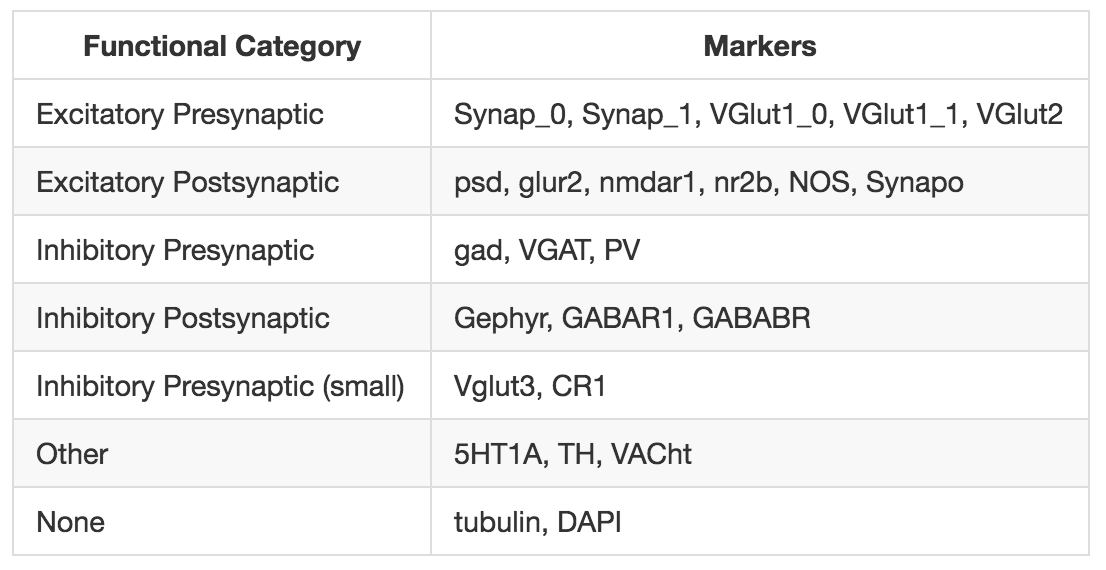
\includegraphics[width=\linewidth]{figures/table1.png}
	\caption{Table 1: Table showing the data collectors providing domain knowledge regarding groupings of the 24 protein markers. Each marker belongs to one of seven functional groupings.}
	\label{fig:table1}
\end{figure}

% Correlation Plot
\begin{figure}
\centering 
\subfigure[]{
	\label{fig:figure1a}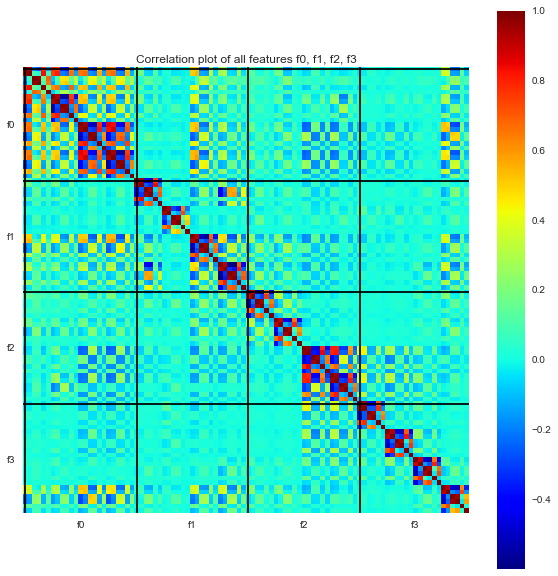
\includegraphics[width=70mm]{figures/corrplot.png}
}
\subfigure[]{
	\label{fig:figure1b}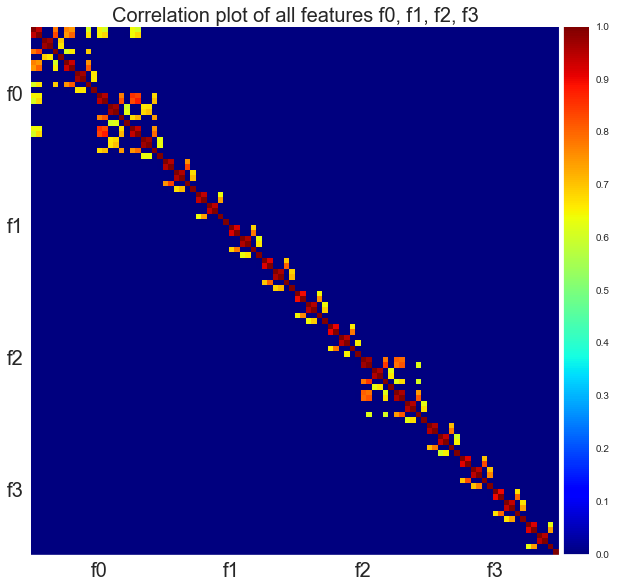
\includegraphics[width=70mm]{figures/thresholdcorrplot.png}
}
\caption{Pairwise correlation plots of the entire feature set, with (a) being the correlation plot without a threshold, and (b) having a threshold of 0.6 applied. All correlations less than or equal to 0.6 were set to 0.}
\label{fig:figure1}
\end{figure}

% f0 Data Check
\begin{figure}
\centering 
\subfigure[]{
	\label{fig:figure2a}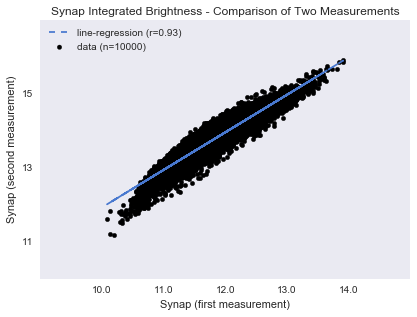
\includegraphics[width=75mm]{figures/data_check01.png}
}
\subfigure[]{
	\label{fig:figure2b}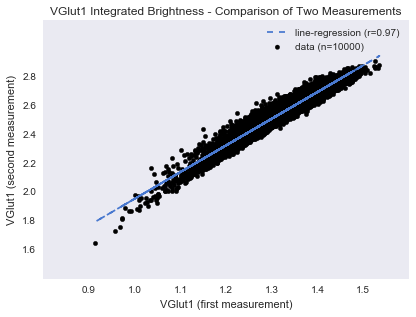
\includegraphics[width=75mm]{figures/data_check02.png}
}
\caption{Pairwise scatter plots of the repeated measurements of Synapsin and VGlut1, showing the integrated brightness.}
\label{fig:figure2}
\end{figure}

% Figure lognormalized BIC plot
\begin{figure}
\centering
\subfigure[]{
	\label{fig:figure3a}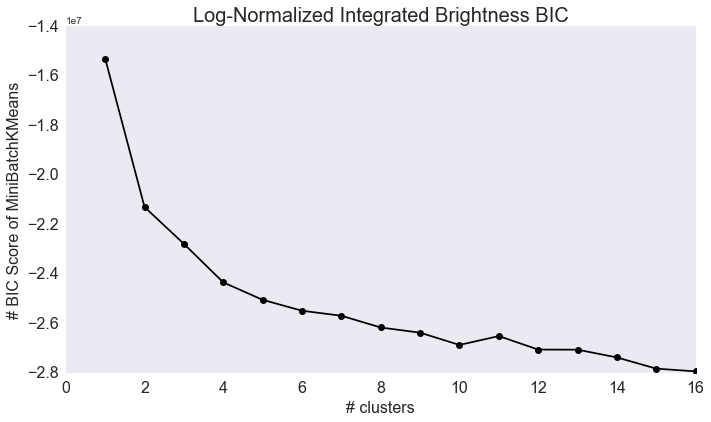
\includegraphics[width=75mm]{figures/exploratory/f0_lognormalized_bicplot.png}
}
\subfigure[]{
	\label{fig:figure3b}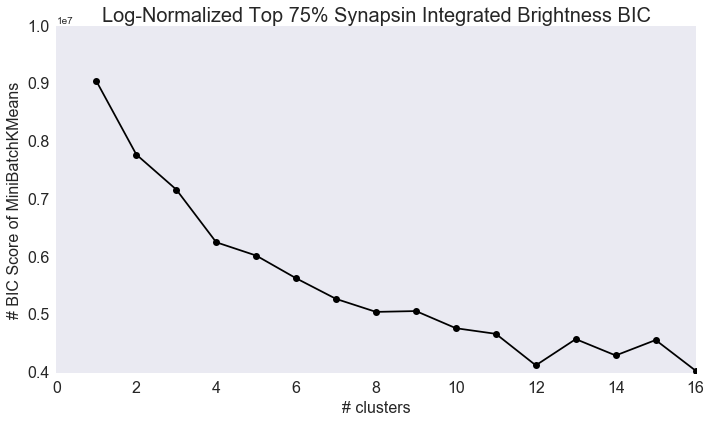
\includegraphics[width=75mm]{figures/exploratory/f0_lognormalized_bottom25_bicplot.png}
}
\subfigure[]{
	\label{fig:figure3c}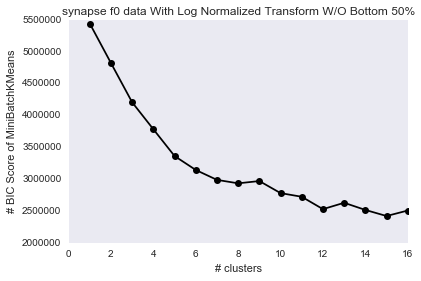
\includegraphics[width=75mm]{figures/exploratory/f0_lognormalized_bottom50_bicplot.png}
}
\subfigure[]{
	\label{fig:figure3d}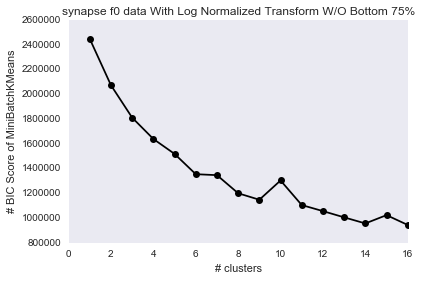
\includegraphics[width=75mm]{figures/exploratory/f0_lognormalized_bottom75_bicplot.png}
}
\caption{Figure (a) showing a BIC plot generated using MinibatchKMeans with a k={1,..,16} on the integrated brightness values. (b,c,d) show the BIC plots with the bottom 25, 50, and 75 percent Synapsin values filtered out respectively.}
\label{fig:figure3}
\end{figure}

% Figure of KMeans=4
\begin{figure}[H]
	\centering
	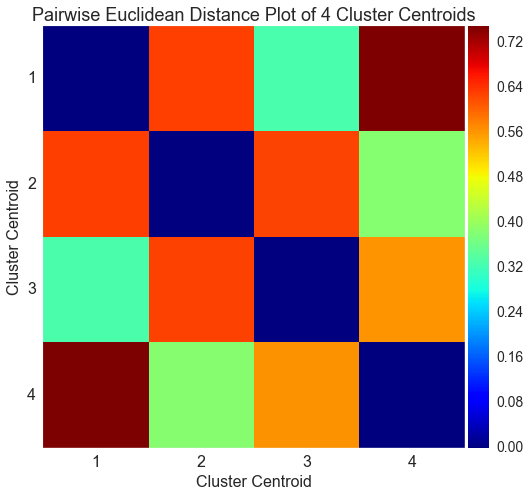
\includegraphics[scale=0.5]{figures/cluster4pairwisedistance.png}
	\caption{KMeans clustering with k=4. Along the diagonal all pairwise distances are equal to 0.0, while the off diagonals show relative euclidean distance. All off diagonals are relatively spaced away from each other with a minimum euclidean distance of ~0.3.}
	\label{fig:figure4}
\end{figure}

% Figure Scree Plots
\begin{figure}
\centering
\subfigure[]{
	\label{fig:figure5a}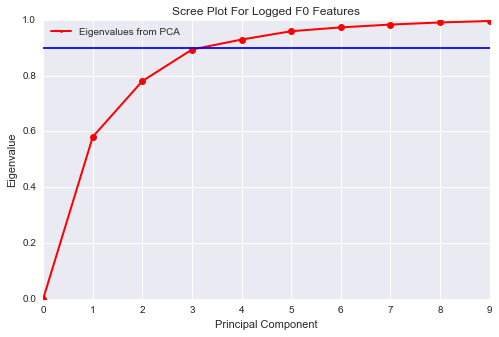
\includegraphics[width=75mm]{figures/exploratory/f0_lognormalized_screeplot.png}
}
\subfigure[]{
	\label{fig:figure5b}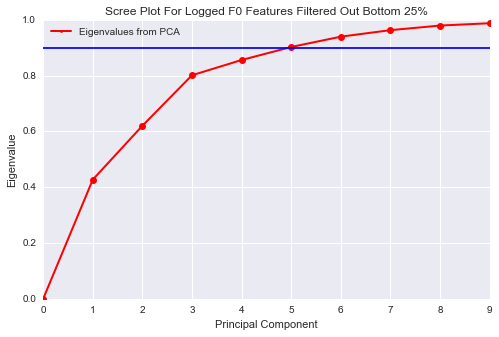
\includegraphics[width=75mm]{figures/exploratory/f0_lognormalized_bottom25_screeplot.png}
}
\subfigure[]{
	\label{fig:figure5c}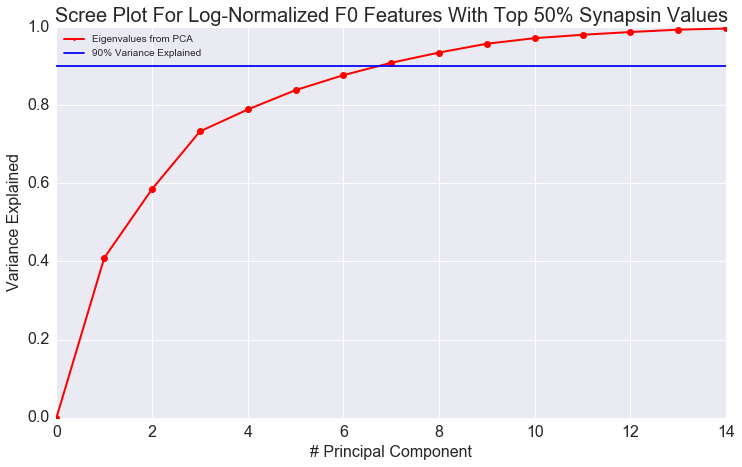
\includegraphics[width=75mm]{figures/exploratory/f0_lognormalized_bottom50_screeplot.png}
}
\subfigure[]{
	\label{fig:figure5d}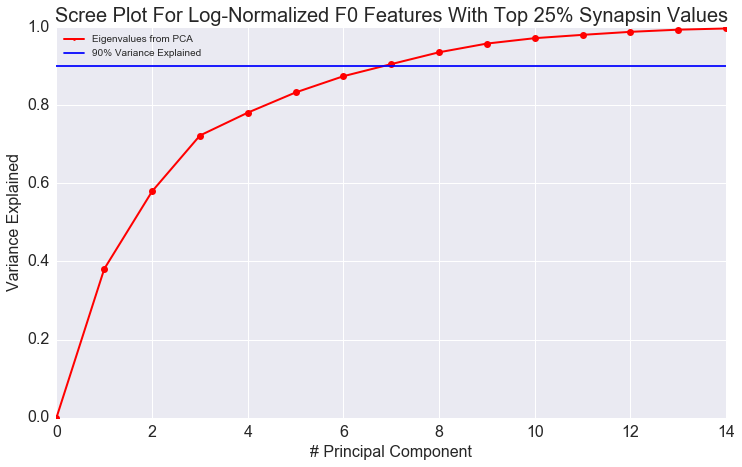
\includegraphics[width=75mm]{figures/exploratory/f0_lognormalized_bottom75_screeplot.png}
}
\caption{Figure (a) showing a scree plot on the entire lognormalized dataset on the integrated brightness values. (b,c,d) show the scree plots with the bottom 25, 50, and 75 percent Synapsin values filtered out respectively. The solid line represents 90\% variance.}
\label{fig:figure5}
\end{figure}

% References Area
\newpage
\small{
	\bibliography{/Users/adam2392/Documents/Bibtex/Synapse_Diversity.bib}
	\bibliographystyle{plain}
}

\end{document}